\FloatBarrier
\subsection{Loading video data}\label{sec:load}
We process the whole night of auroral image data offline.
As described in section~\ref{sec:currentpc}, commodity computer hardware currently available allows recording all night.
On-line processing will necessarily be time-constrained, and if some unexpected event occurs (e.g. meteor, vehicle reentry) the possibly unique data would be lost as the discrimination algorithm is not tuned for such an event.

For reduced processing time, one can choose to sample every N\textsuperscript{th} frame set.
Deciding which interval to sample at is driven by the need to sample the entire night's data and extract interesting frames before it's time to record again for the next night.
Although DAW events evolve on sub-second time scales, there are generally several DAW sub-events happening in parallel and serially over 5..\unit[15]{s} intervals, with several such groups of events occurring within 1..\unit[5]{min.}
The bounds on discrimination algorithm data loading cadence $T_L$ in seconds is thus bounded by
\begin{equation}\label{eq:loadint}
T_0 < T_L < T_1.
\end{equation}
Empirically, an Intel i7 Ivy Bridge CPU yields $N \gtrsim 20$ and with camera kinetic rate $T_K=\unit[20]{ms}$, $T_0 \sim \unit[400]{ms}$.
Given typical event duration $\unit[5]{s} \lesssim T_E \lesssim \unit[15]{s}$, $T_1 \sim \unit[2]{s}$.
Thus \eqref{eq:loadint} becomes
\begin{equation}\label{eq:actload}
0.4 < T_L < 2.
\end{equation}
As computer hardware capability increases with future CPU generations, $T_0$ becomes smaller and/or more advanced discrimination algorithms may be employed.

The images are stored in a raw binary stream containing a fixed-length footer containing a sequence number and other user-chosen per-frame metadata.
DMC and HiST phase 1 used a four byte footer for this purpose.
For simplicity, the experiment configuration is stored in a standard XML file.
The raw binary file will be more than \unit[1]{TB} in size for a whole night recording, so for ease of download and user experience auroral events of interest are repacked into an losslessly compressed HDF5 format file.
The HDF5 file is chunked, one image per chunk for fastest reading, combined with metadata like the format used by the Madrigal geospace data repository \citep{madrigal} and uploaded to Zenodo.

Auroral image histograms are not adequate to discriminate on alone since they do not contain sufficient information about the morphology. 
The ground-observed brightness of aurora is highly dependent upon viewing angle and the arrangement of the aurora along a particular viewing angle as described by~\eqref{eq:bint}.
An example auroral histogram on a clear viewing night with a few bright stars and a discrete arc away from magnetic zenith is shown in Figure~\ref{fig:diffimhist}.
\begin{figure}\centering
    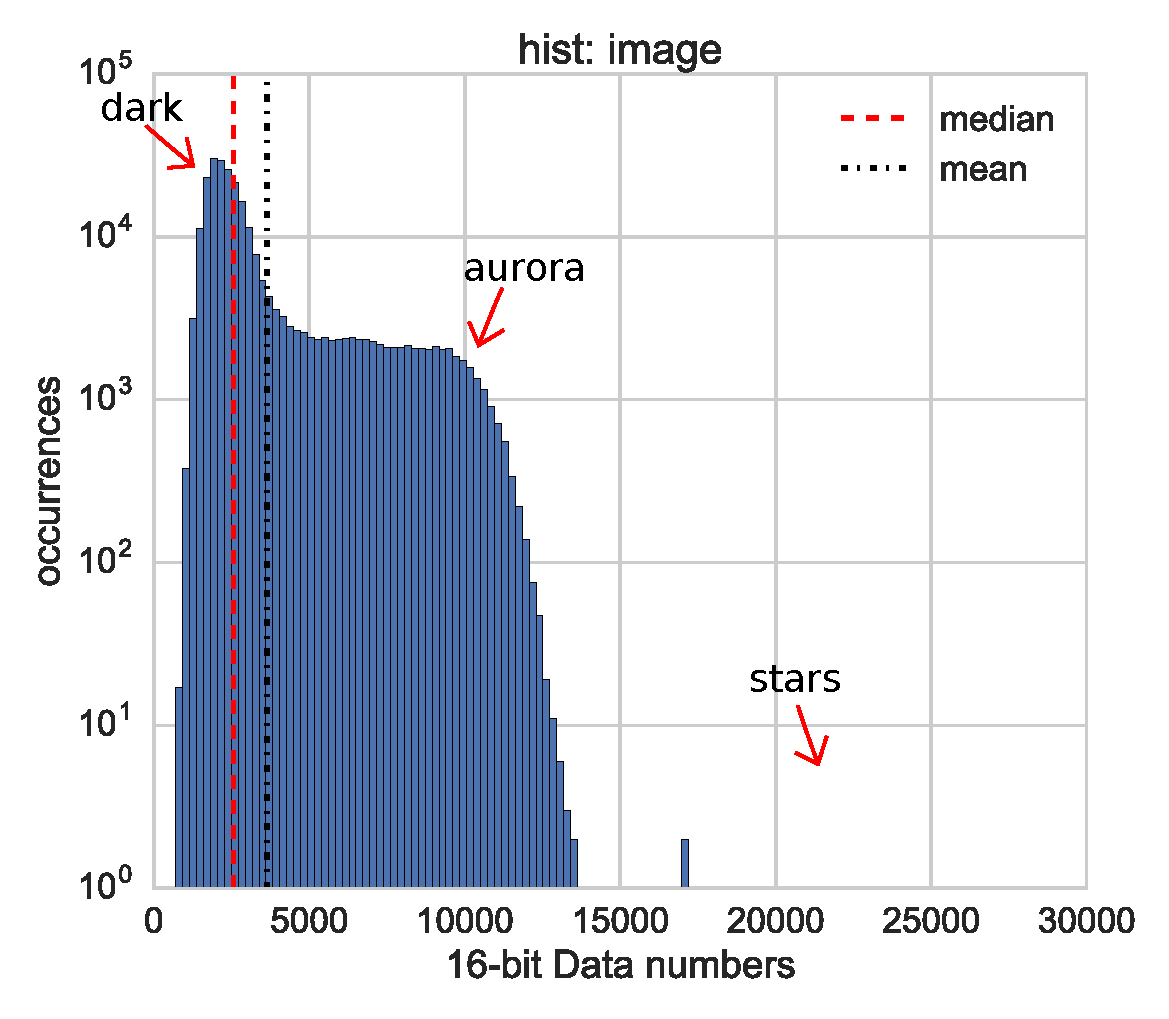
\includegraphics[width=0.7\linewidth]{gfx/diffuse-imhist}
    \caption{Histogram of discrete arc away from magnetic zenith.}\label{fig:diffimhist}
\end{figure}
Due to photon-stared low auroral video SNR, there is no clear separation between auroral intensity values and background noise, thus even adaptive intensity threshold algorithms fail.

\FloatBarrier
\subsection{Image Noise Filtering}\label{sec:filtnoise}
Noise reduction is a common preprocessing step, particularly in auroral video where SNR is often low and the target is smooth as a result of diffusion of the particle stream scale for $\unit[100]{m} > B_\perp > \unit[10]{m}$ in the ionosphere.
The 2-D Wiener filter is often chosen for auroral video noise reduction as the Wiener filter is MMSE-optimal for additive noise \citep{vaseghi2000} and in auroral video sensor noise is often strong due to low video SNR.
The more advanced edge-preserving noise filters often of interest for terrestrial objects in commercial and personal photography are not necessarily relevant to auroral video since the physics dictate that the targets of interest are always spatially smooth.
In this sense, a simpler filter such as a spatial low-pass filter or Gaussian blur are less computationally demanding while meeting the smoothing criterion.

We assume the only degradation of the image is due to noise in the camera image sensor chip, since the camera is mounted stably and normally samples in excess of the auroral Nyquist rate.
By these assumptions, the noise-free analog image $\mathscr{I}$ projected onto the semiconductor imaging array is corrupted by additive noise ensemble $\mathcal{N}$ into observable digital image $I$
\begin{equation}\label{eq:imgmapsimple}
I(i,j) = \mathscr{F}\lbrace\mathscr{I}(x,y)\rbrace + \mathcal{N}(i,j).
\end{equation}
$(x,y)$ are Cartesian coördinates in $\mathbb{R}^2$, where $\mathbb{R}$ is the set of real numbers.
The pixel centers $(i,j)$ of $I$ are described by tuple pairs drawn from Cartesian space $\mathbb{Z}^2$, where $\mathbb{Z}$ is the set of all integers.
By convention, $(x,y)$ and $(i,j)$ are used interchangeably where the context is clear.
$\nu$ is the superposition of several stochastic noise processes in the image sensor.
$\mathscr{F}\lbrace\cdot\rbrace$ represents the sampling of the digital image sensor, the mapping from analog image formed in the imaging plane to digital image in camera memory.
Without loss of generality, in a noise-free system the imaging chip sampling process is modeled as
\begin{equation}\label{eq:anadig}
I(i,j) =\mathscr{F}\lbrace\mathscr{I}(x,y)\rbrace = \int_\lambda \int_{(x,y)\in \mathbb{R}^2} R(\lambda)F(x,y)\mathscr{I}(x,y) \textrm{d}\mathbb{R} \textrm{d}\lambda
\end{equation}
where $I$ is linearly quantized into 65,536 levels with 16 bits in a modern scientific camera.
$F \in [0,1]$ is the dimensionless fill factor, normally near unity with modern scientific imaging chips.
$R(\lambda)$ with units ampere/watt is the responsivity of the imaging chip as a function of wavelength $\lambda$, relating the photoelectron production in the imaging chip semiconductor material versus incident photon flux \citep{saha2015}
\begin{equation}
R(\lambda) = \eta_e(\lambda) \frac{e}{\hslash \nu}.
\end{equation}
where $\eta_e$ is the quantum efficiency of the imaging sensor (typically 0.5 for sCMOS and 0.9 for EMCCD at visible wavelengths), $e$ is electron charge, $\hslash$ is Planck's constant and $\nu$ is the frequency of the light.


Since the EMCCD or sCMOS sensor temperature is hardware control loop stabilized to order $\unit[0.01]{^\circ C}$, each local pixel neighborhood may be considered wide-sense stationary (WSS) and ergodic \citep{kuan1985}.
\citet{hunt1980} argued that even though the image mean is not globally ergodic, the autocovariance could be ergodic.
In general the whole image is \textit{not} WSS or ergodic, but the localized WSS/ergodic Wiener filter described by \citet{kuan1985,jin2003} allow expedient Wiener-type filtering, particularly where the image histogram has a Gaussian-like probability distribution function (pdf) \citep{jin2003}.

Particularly for smoothly varying auroral images, the local mean $\mu_l(x,y)$ of a noise-free image describes the brightness of the $m \times n$ pixel neighborhood $S_{xy}$.
\begin{equation}\label{eq:localmean}
\mu_l(x,y) = \frac{1}{mn} \sum_{(i,j)\in S_{xy}} I(i,j)
\end{equation}
$\mu_l(x,y)$ might be thought of as representing the low-frequency structure of an image class \citep{hunt1980}.
%In fact,~\eqref{eq:localmean} can be used as a blurring filter itself.
A mask size of $7\times7$ was empirically found to give adequate performance for typical EMCCD and sCMOS auroral video.
\begin{equation}
\textbf{M}=
\begin{bmatrix} 
1 & 1 & 1 & 1 & 1 & 1 & 1 \\ 
1 & 1 & 1 & 1 & 1 & 1 & 1 \\ 
1 & 1 & 1 & 1 & 1 & 1 & 1 \\ 
1 & 1 & 1 & 1 & 1 & 1 & 1 \\ 
1 & 1 & 1 & 1 & 1 & 1 & 1 \\ 
1 & 1 & 1 & 1 & 1 & 1 & 1 \\ 
1 & 1 & 1 & 1 & 1 & 1 & 1  
\end{bmatrix}
\end{equation}

By extension, the local variance $\sigma_l^2(x,y)$ of a noise-free image describes the contrast and distinct structure within the pixel neighborhood.
Using the definition of variance for general random variable $\xi$ with mean $\mu$
\begin{equation}
\sigma^2 = E[\xi^2] - \mu^2 = E[\xi^2] - (E[\xi])^2
\end{equation}
we obtain from~\eqref{eq:localmean}
\begin{equation}\label{eq:localvar}
\sigma_l^2(x,y) = \frac{1}{mn} \sum_{(i,j)\in S_{xy}} I^2(i,j) - \mu_l^2(x,y)
\end{equation}

\citet{kuan1985} introduced the nonstationary mean and nonstationary variance (NMNV) Wiener filter
\begin{equation}\label{eq:nmnv}
\widehat{\mathscr{I}} = \mu_l + \frac{\sigma_l^2 - \sigma_n^2}{\sigma_l^2}(I-u_l)
\end{equation}
where $\sigma_n^2$ is the noise variance.
In SciPy \citep{scipy}, the efficient C-code implementation of~\eqref{eq:localmean} and~\eqref{eq:localvar} are obtained by cross-correlation with unity mask $\textbf{M}$ of the desired shape to compute~\eqref{eq:nmnv}.
The NMNV Wiener filter has been more than adequate for an initial denoising of the video.

Flat fielding (removal of image vignetting) and background subtraction (accounting for hot or cold pixels and DC sensor bias) are a standard part of auroral image processing, particularly for a tomographic system.
After flat fielding and background subtraction, the image noise is i.i.d., WSS, and ergodic. 
Thus a noise sample from a non-auroral image periodically allows a good noise estimate for the Wiener filter.
In section~\ref{sec:of} we continue this heuristic approach when comparing a pixel neighborhood \textit{temporally}.


\subsection{Auroral Optical Flow Estimation}\label{sec:of}
Previous efforts \citep{blixt2006} used an optical flow estimator directly to estimate parameters of finely structured aurora, including structures associated with inverted-V and Alfvénic driven aurora.
Robust flow estimators flag areas where constraints are broken \citep{black1996}.
However, auroral events of interest often have video SNR approaching zero, and typical optical flow techniques are highly sensitive to noise due to the spatial derivatives employed.
Typical optical flow algorithms assume high SNR video, and so robust estimator constraints will simply be broken throughout the video frames on non-bright auroral video. 

A general method applicable to auroral video of any SNR, and particularly low SNR in order to capture the most possible events with acceptable false alarm rate is needed.
We do \textit{not} want to rely on seeing strong backscatter in the ISR from turbulence as that would bias observations toward only those with strong ISR backscatter.
The key criterion is sensitivity at low false alarm rate for $\textrm{SNR}\ll 2$ aurora.
The filtering of section~\ref{sec:filtnoise} mitigates the worst of the noise, but additional post-processing steps are needed, particularly for low SNR auroral video.
Optical flow estimators \citep{hornschunck} have been implemented in numerous languages including Python \citep{hscode} along with associated morphological and filtering operations.
%FIXME consider specific examples of Black vs Horn-Schunk vs Lucas Kanade

A typical scientific camera is a power sensor array of $512 \times 512$ or more pixels with 16-bit ADCs yielding data numbers $\in [0..65535]$.
Quantum efficiencies in the 50\% range for sCMOS and 90\% range for EMCCD yield vast weak auroral SNR advantages over early 8-bit digital cameras and the 5..10\% quantum efficiency obtained from the pinnacle of digital-assisted emulsion plate analog imaging \citep{parker1993}.
Even the narrowest auroral arcs observed with a medium field of view, say $10^\circ$ will cover several pixels for the E-region aurora of interest.
For a $10^\circ$ FOV lens/camera pair, each pixel of a $512\times512$ pixel camera aimed at magnetic zenith has approximately $10/512 = 0.0195^\circ$ spacing/pixel.
A \unit[100]{m} wide auroral arc with peak intensity at \unit[110]{km} near magnetic zenith subtends $\tan^{-1}(0.1/110) = 0.0521^\circ$, so the camera would see about 3..5 pixels covered by this arc, considering the point spread function (PSF) of the optical system.
These values represent the typical HiST optical setup as denoted in Table~\ref{tab:camerareshist}.
\begin{table}\centering
\caption{HiST camera resolution parameters.}\label{tab:camerareshist}
    \begin{tabular}{cccc}
        \toprule
        camera & binned resolution (pixels) & resolution ($B_\perp$ meters) & frames/sec\\
        \midrule
        iXon 879 & $512 \times 512$ & 37.5 & 30  \\
        iXon 897 & $512 \times 512$ & 37.5 & 50 \\
        \bottomrule
    \end{tabular}
\end{table}

The DMC instrument uses an Andor Neo sCMOS camera with $2560 \times 2160$ pixels and a Marshall \unit[140]{mm} lens, yielding a $6^\circ \times 8^\circ$ FOV.
This implies resolution of $6/2160 = 0.00278^\circ$/pixel, so a \unit[100]{m} wide arc covers about 19..22 pixels, considering PSF.
The reduced sensitivity of the sCMOS camera is partially offset by binning, that is, grouping of adjacent pixels into macropixels.
The averaging of the i.i.d. noise across the pixels improves SNR to first order by a factor $\sqrt{B_xB_y}$ where $B_x, B_y$ are the binning factors along the columns and rows of the image sensor respectively.
Typically for DMC experiments, $4 \times 4$ binning was used, yielding videos with the characteristics of Table~\ref{tab:cameraresdmc}.
The other camera used for context in the DMC system is an Andor iXon with a Kowa lens yielding a $50^\circ$ FOV, with parameters in Table~\ref{tab:cameraresdmc}.
These parameters are experimentally determined as per section~\ref{sec:hist}, the specification sheets and software ratings must be derated for all-night auroral capture.
\begin{table}\centering
    \caption{DMC camera resolution parameters.}\label{tab:cameraresdmc}
    \begin{tabular}{cccc}
        \toprule
        camera & binned resolution (pixels) & resolution ($B_\perp$ meters) & frames/sec\\
        \midrule
        iXon 897 & $512 \times 512$ & 187.5 & 30  \\
        Neo & $640 \times 540$ & 21.3 & 50 \\
        Neo & $320 \times 270$ & 42.6 & 100 \\
        \bottomrule
    \end{tabular}
\end{table}

Spatial derivatives for noise-filtered auroral video have magnitude
\begin{equation}
0 \leq |D| \leq \max(I)
\end{equation}
where $\max(I)$ is the maximum intensity in an image pair.
Stars will also have spatial derivatives somewhat larger than aurora, defined by the PSF of the optical system and seeing conditions.
An example optical flow measurement is shown in Figure~\ref{fig:optflowdiff}.
\begin{figure}\centering
    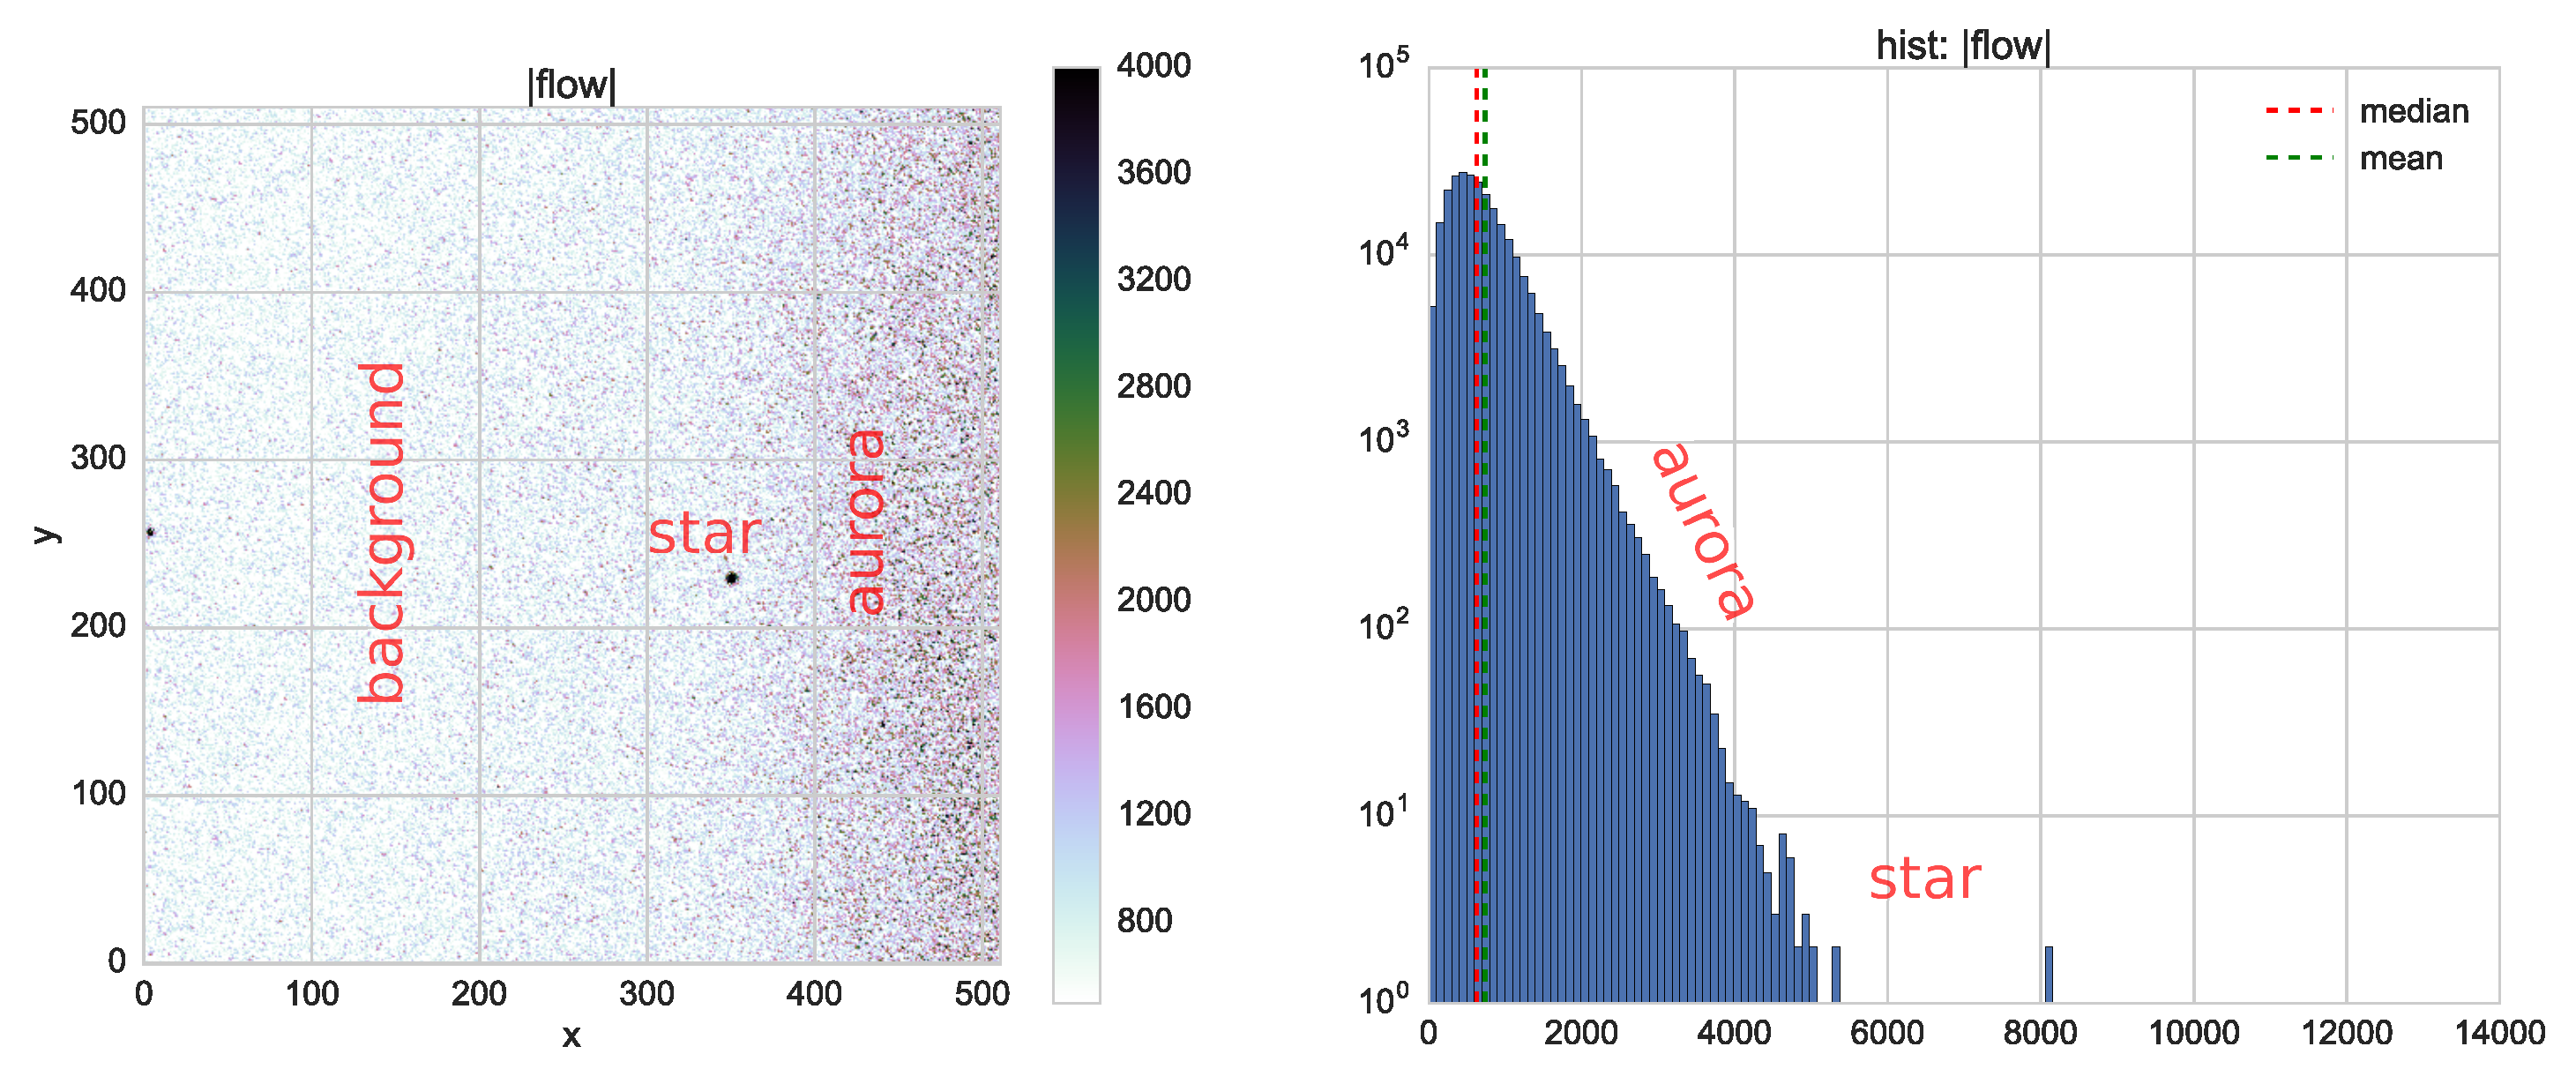
\includegraphics[width=\linewidth]{gfx/optflow-diffuse}
    \caption{(a) dense optical flow estimate using same image data as in Figure~\ref{fig:diffimhist}}\label{fig:optflowdiff}
\end{figure}
As with the image data histograms, the spatial derivative alone is not enough to distinguish interesting aurora from stars, clouds, and satellites.

Given the desire to exploit spatially correlated behavior of a discrete auroral arc, one typical approach is to reduce the resolution of the input image.
In this application however, to meet the spatial Nyquist criterion, we do not have the freedom to significantly reduce raw image resolution for risk of smearing out the closely spaced arcs that are vital to the purpose of HiST as seen by the parameters in Table~\ref{tab:camerareshist}.
Thus to exploit the locally collective behavior of aurora, particularly discrete aurora, optical flow estimation is chosen as a first processing step.
Farneback is a dense optical flow estimation algorithm that has proven suitable for the task.

%INWORK describe farneback parameters
The estimated optical flow $(U,V)$ is passed to the next module for segmentation.


\subsection{Foreground Segmentation}\label{sec:seg}
The HiST system is configured with camera gain set to maximize dynamic range under typical observing conditions.
The gain of the cameras are fixed for a given HiST experiment since tomographic analysis by definition is highly sensitive to relative intensity calibration of the cameras.
The SNR of observable auroral arcs cover about nine orders of magnitude with 16-bit scientific cameras by
\begin{equation}
20\log_{10}\left(2^{16}\right) = \unit[96.3]{dB}
\end{equation}
less ENOB, amplifier noise, readout noise, clock noise, \&c.
Thus a constant false alarm rate (CFAR) \citep{cfaroptical} algorithm was devised based on the noisiness of the video.
False negatives will increase as video SNR decreases, but this is necessary to avoid constant false positives during the vast majority of the time when Alfvénic aurora is not within 5 degrees of magnetic zenith for the HiST system.
The CFAR algorithm employed consists of two user-defined constants ${C_0,C_1}$ for lower (clouds/diffuse aurora suppressing) and upper (noise \& star-suppressing) decision thresholds.
The decision outcome is stored in binary matrix $A$ of the same dimensions as a single image.
\begin{equation}
A = T_0 < \sqrt{U^2 + V^2} < T_1
\end{equation}
Each element of $A$ maps 1:1 to a digital video image pixel $I(x,y)$ by \eqref{eq:anadig} corresponding to the latest frame of video processed.


%\subsection{Despeckle Filter}\label{sec:despeck}
%A 2-D median filter is applied to reduce the presence of impulse-like noise induced by the noisy original image.
%In a general 2-D median filter, pixel values are replaced with the median of the $N$ neighbor pixels in both directions.
%Pixel groups must have at least $N \times N-1$ pixels along the other axis for $N-2 \times N-3$ pixel group to ``survive'' the median filter operation as illustrated in Figure~\ref{fig:medfilt}.
%The net effect is to remove individual binary pixels before further processing steps.

\subsection{Morphological Erosion}\label{sec:erode}
The morphological erosion step removes isolated pixels like a median filter, and additionally removes groups of pixels and protuberances too small to fit the structuring element (SE).
If such a region cannot completely contain the SE, that region is eliminated from the binary image. 
Morphological erosion is a set process where image $A$ is operated on by translating structuring element (SE) $B$ over all $A$ 
\begin{equation}\label{eq:erosion}
A \ominus B = \lbrace z|(B)_z \subseteq A \rbrace = \lbrace z | (B)_z \cap A^c = \oslash \rbrace
\end{equation}
where $(B)_z$ represents the translation of $B$ across all $A(i,j)$.
\eqref{eq:erosion} says that as $B$ is scrubbed over all of $A$ with integer-based translation $z$, keep only those values where $B$ is \textit{entirely} contained in $A$.
%If a region can contain the SE, then as the SE is slid around inside the region, the pixels “touched” by the center pixel of the structuring element are preserved.
A cartoon depiction of erosion with a rectangular SE in orange and the resulting one-pixel wide red line in Figure~\ref{fig:erode}.
Notice at the chamfered ends of the pixel region, there was no output because the SE did not fit entirely within that region.
\begin{figure}\centering
	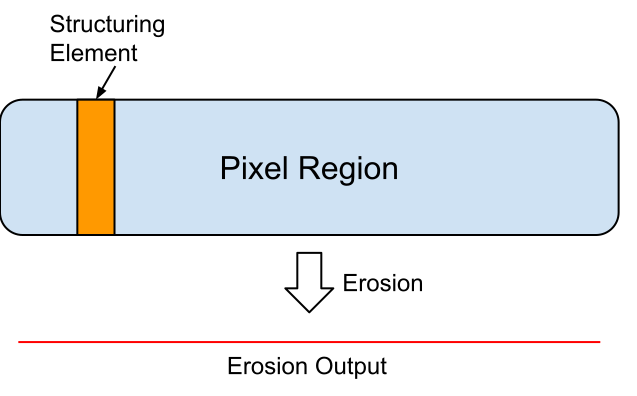
\includegraphics[width=0.8\linewidth]{gfx/erode}
	\caption{Example of morphological erosion with a rectangular structuring element. 
		Outside blue region is assumed identically zero.}
	\label{fig:erode}
\end{figure}
A comparison of the median filter operation versus the erosion operation is illustrated in Figure~\ref{fig:medfilt}.
\begin{figure}\centering
    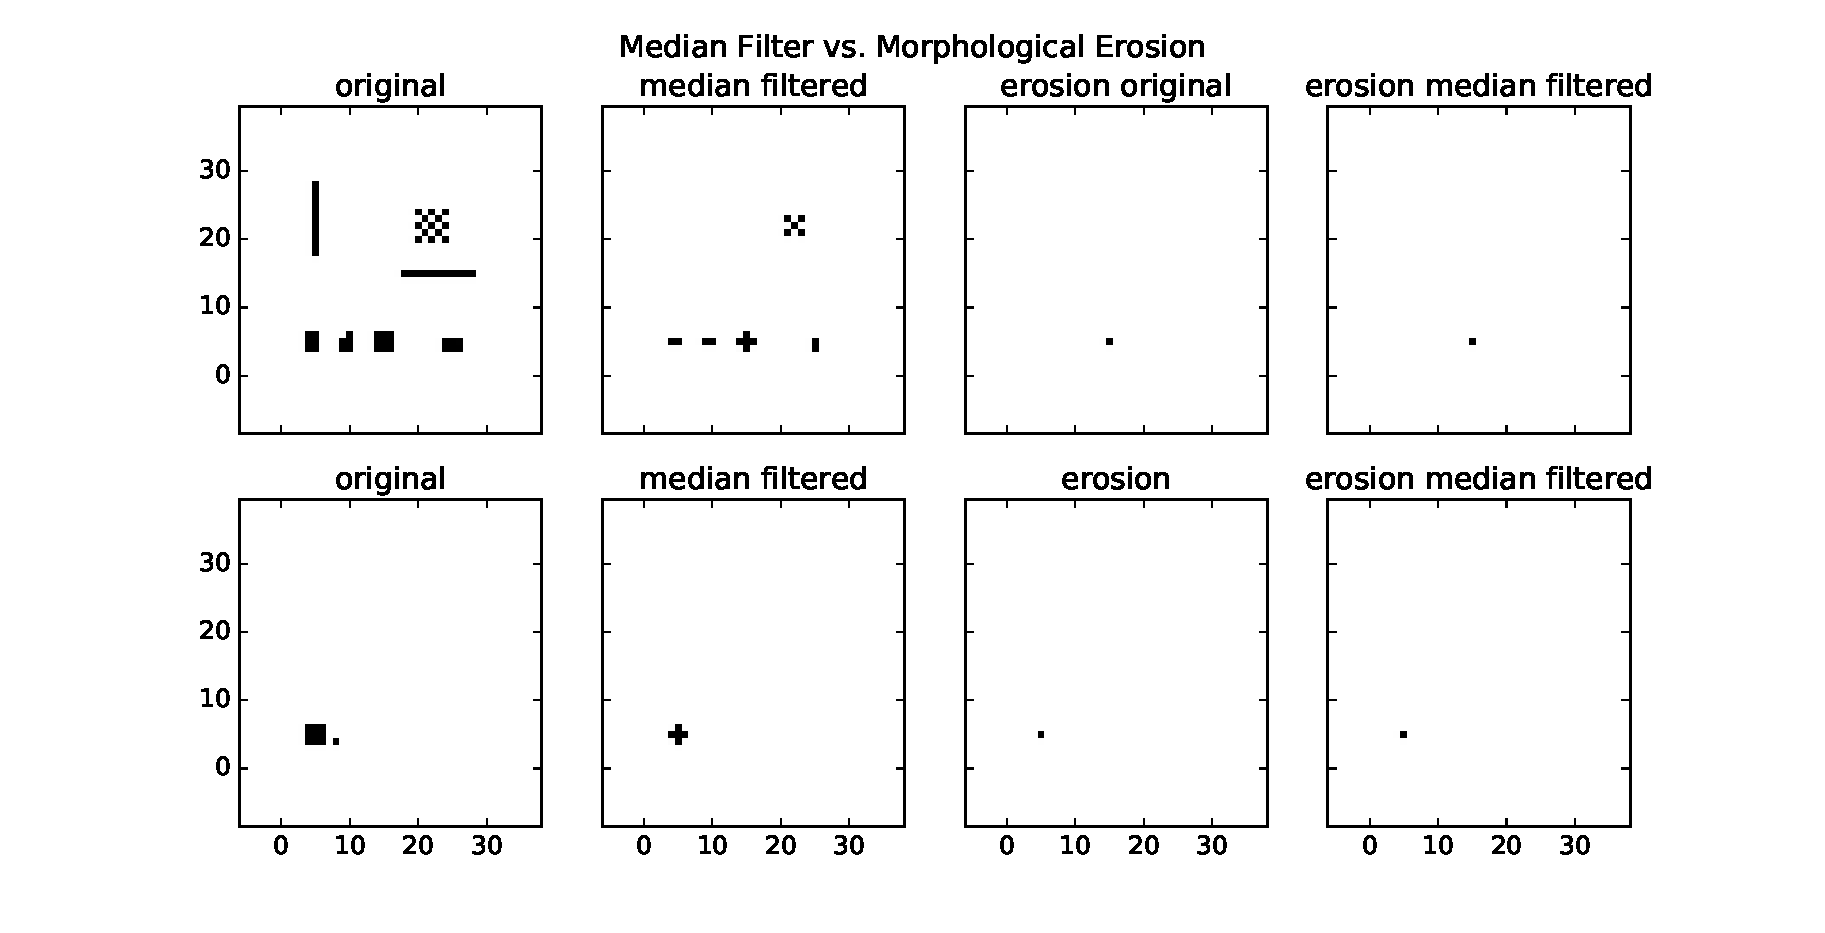
\includegraphics[width=0.75\columnwidth]{gfx/medfilt}
    \caption{Binary Median Filter versus Morphological Erosion example, showing how at least $N \times N-1$ pixels are required to ``survive'' the operation.}\label{fig:medfilt}
\end{figure}
This step provides much of the denoising one might otherwise apply at substantial computational expense earlier in the process, which is important for rapid processing of terabytes of data whether online or offline.

\subsection{Morphological Dilation}\label{sec:dilate}
While erosion removes thin or isolated features in an image, dilation is a thickening operation that connects small gaps in $A$ according to $B$
\begin{equation}\label{eq:dilate}
A \oplus B = \bigcup_z (B)_z.
\end{equation}
Imagine a peg in the center pixel of the structuring element--the result of dilation is that any place touched by any pixel of the structuring element as the peg is translated within $A$ is declared binary True.
A cartoon example of morphological dilation is shown in Figure~\ref{fig:dilate}. 
\begin{figure}\centering
    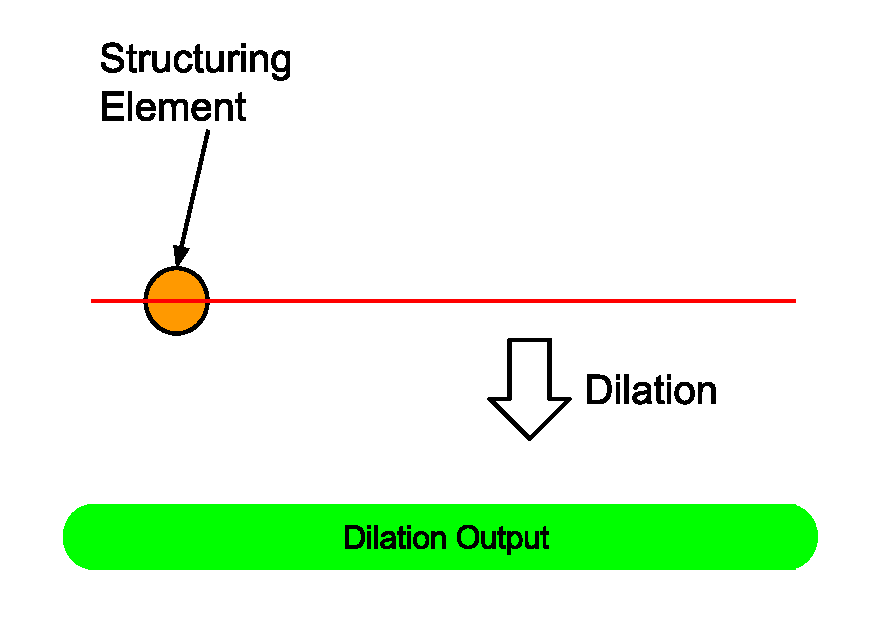
\includegraphics[width=0.7\linewidth,trim=10 0 10 0,clip]{gfx/dilate}
    \caption{Dilation example with orange 5 pixel disk SE. 
            Dilation output is green chamfered bar 5 pixels wide due to SE and one-pixel wide input.}\label{fig:dilate}
\end{figure}
Note that even if the red line in Figure~\ref{fig:dilate} had a break up to one-half the diameter of the structuring element, the continuous green form seen at the bottom of Figure~\ref{fig:dilate} would result. 

\subsection{Morphological Opening}
Morphological opening is an idempotent set operation expressed by erosion \eqref{eq:erosion} followed by dilation \eqref{eq:dilate}.
\begin{equation}\label{eq:open}
A \circ B = \left(A \ominus B \right) \oplus B.
\end{equation}
Observe the rounded corners in the green output of the opening example in Figure~\ref{fig:opening}.
\begin{figure}\centering
    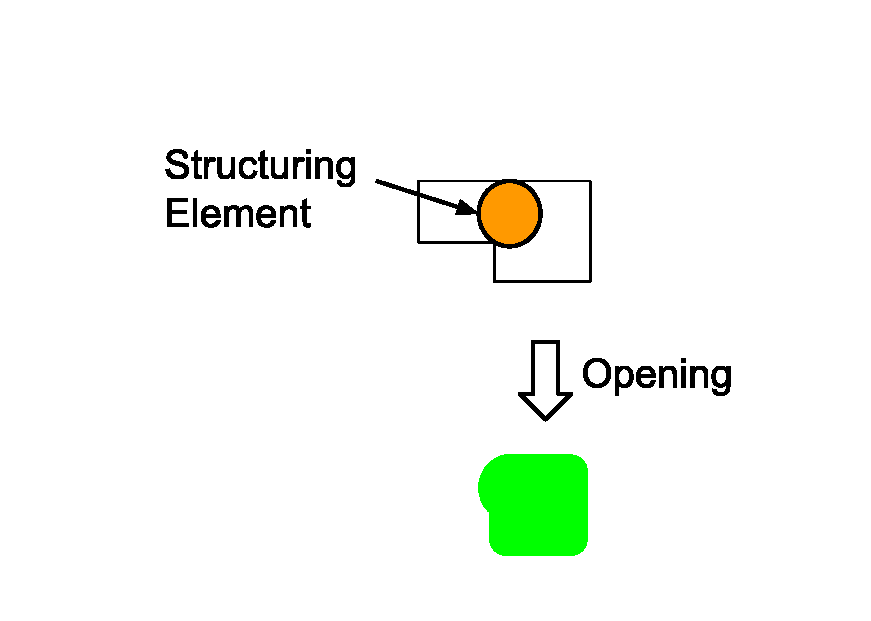
\includegraphics[width=0.7\linewidth,trim=70 20 50 50,clip]{gfx/open}
    \caption{Opening example with disk SE. Opening output is green rounded rectangle.}\label{fig:opening}
\end{figure}
The rounded protrusion at the upper left represents the partial fitting of the SE into the notch into the input $A$.
Heuristically, erosion retains pixels where the center of the SE touches when the SE fits within the region $A$.
Opening keeps all the pixels the SE touches when the SE fits within $A$.

\subsection{Morphological Closing}\label{sec:close}
Morphological closing is an idempotent set operation expressed by dilation \eqref{eq:dilate} followed by erosion \eqref{eq:erosion}
\begin{equation}\label{eq:close}
A \bullet B = \left(A \oplus B \right) \ominus B.
\end{equation}
Closing is heuristically represented by passing the SE completely outside and along the exterior-like rolling the disc SE in Figure~\ref{fig:closing} and filling in gaps to meet the SE.
\begin{figure}\centering
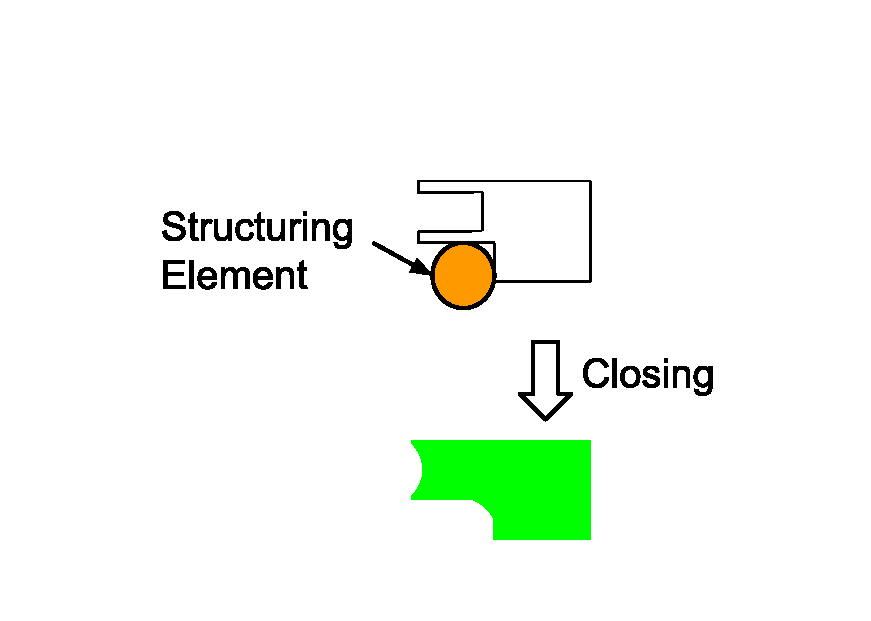
\includegraphics[width=0.7\linewidth,trim=50 0 50 0,clip]{gfx/close}
\caption{Closing example with orange disk SE. Closing output is green concave shape.}\label{fig:closing}
\end{figure}
Morphological closing fills in interior oases that may have occurred due to noise or random intensity behavior at the optical flow thresholding step.
This is physically justified by that aurora is not filled with small holes.
The smallest plausible auroral feature size is $\gg$ 1 pixel for the 9 degree field of view chosen for each HiST camera.
The filling operation implemented by closing is important for the next step which qualifies Alfvénic arc plausibility based on the amount of aurora in view that is moving together.

\subsection{Connected Components Criterion}\label{sec:blob}
Alfvénic aurora is likely to occur as a long sinuous continuous thin feature in the field of view.
The Alfvénic arc may split or flame and intensity may be large or small.
We choose as our criteria a region of thin, rapidly moving aurora of more than 100 contiguous pixels.
At this time we do not impose a shape criteria as this may discard some of the wide variety of shapes Alfvénic aurora can take on.
Such a specific morphology classifier would be a future subsequent step.

We declare as connected any region of contiguous 8-connected pixels.
8-connected neighbors mean any pixel touching a face or corner of another pixel as depicted in Figure~\ref{fig:8conn}.
\begin{figure}\centering
	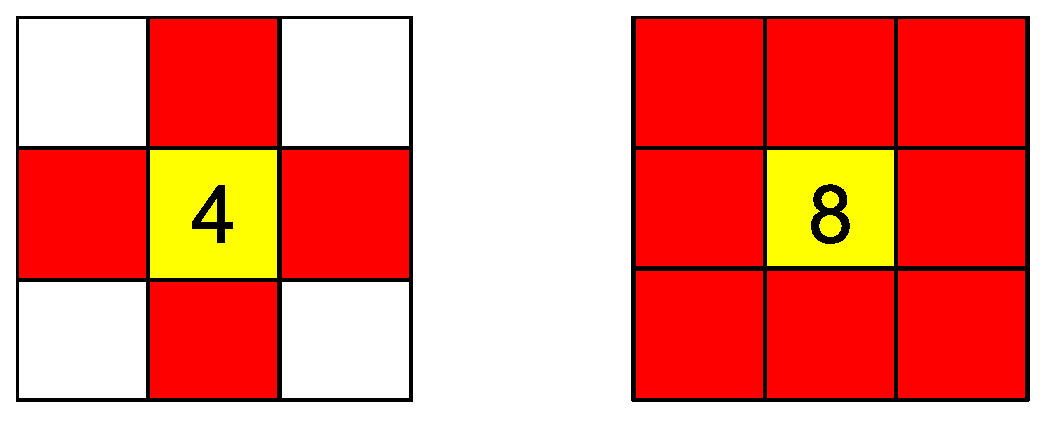
\includegraphics[width=0.8\linewidth,trim=0 0 10 0,clip]{gfx/4conn8conn}
	\caption{Left: 4-connected neighbor pixels. Right: 8-connected neighbor pixels.}\label{fig:8conn}
\end{figure}
Connected component analysis (CCA) computes the size of the oriented minimum bounding box containing the convex hull of an 8-connected pixel region representing the declared foreground (target) pixel \citep{gonzalezwoods}. 
The cartoon in Figure~\ref{fig:connblob} of the convex hull (outlined in purple) of connected pixels is enclosed by the minimum bounding box (outlined in green).
\begin{figure}\centering
	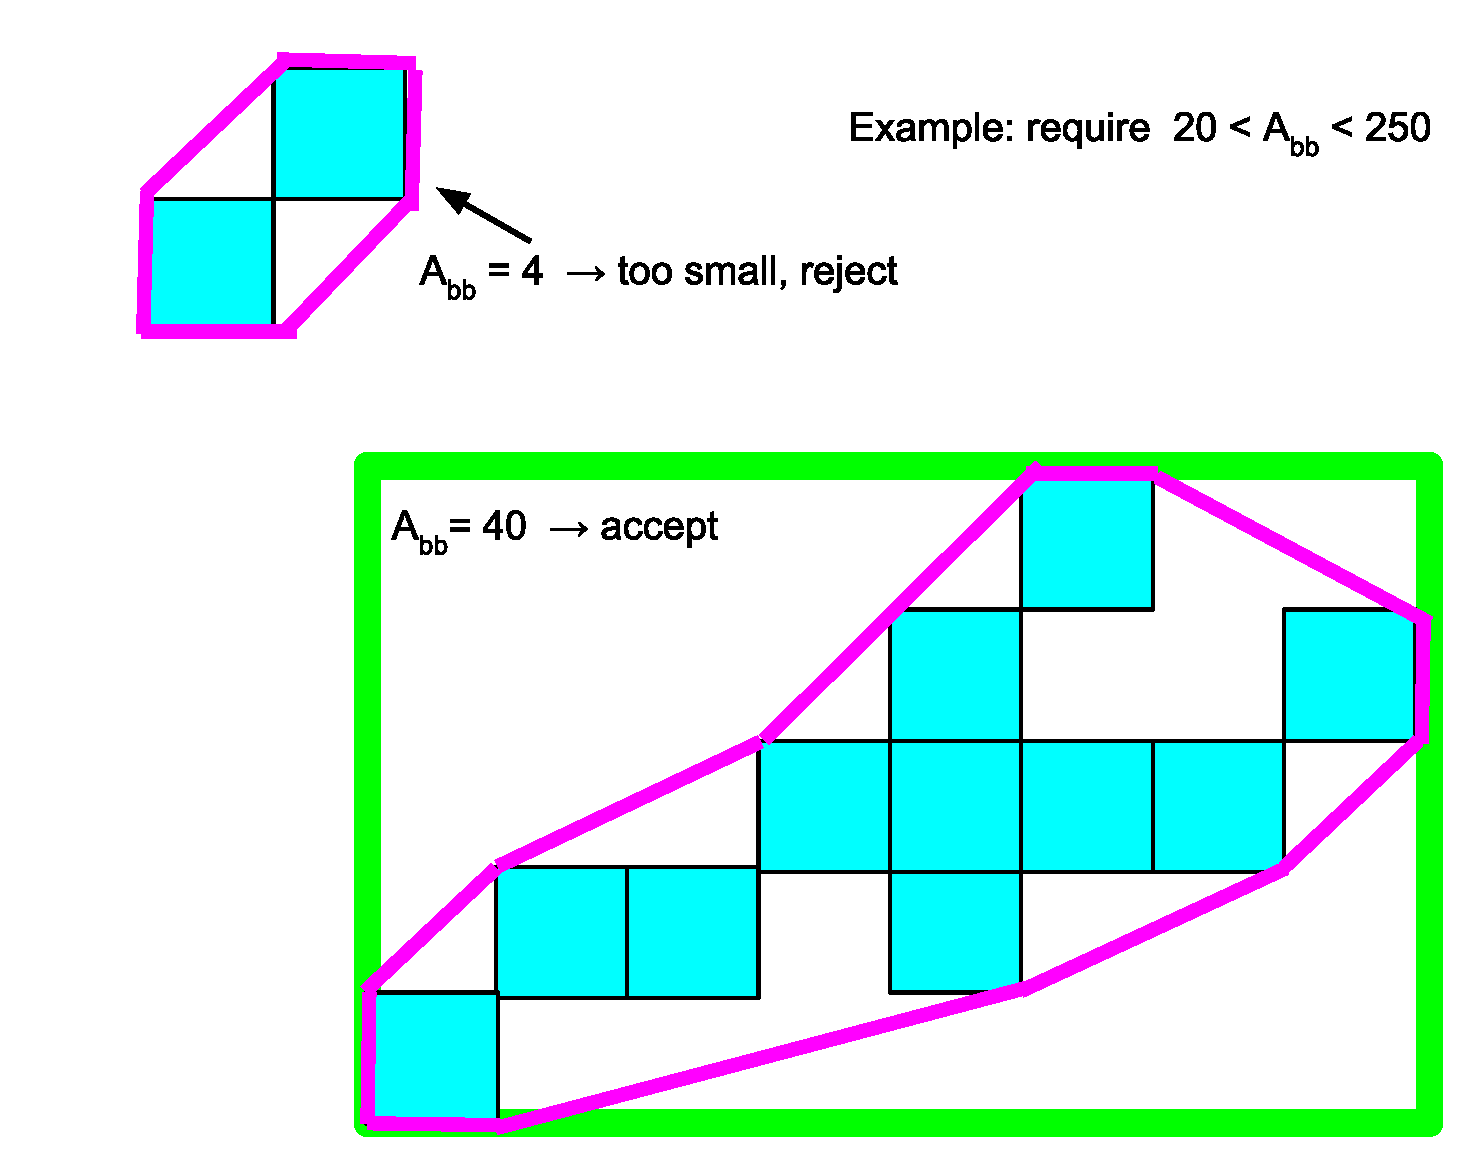
\includegraphics[width=\linewidth,trim= 10 0 10 0,clip]{gfx/connblobcartoon}
	\caption{Example of CCA--upper left pixel group is rejected as having too small convex hull.  Lower right pixel group enclosed in green bounding box is accepted as having sufficiently large convex hull.}\label{fig:connblob}
\end{figure}
Observe how the upper left group of connected pixels has a convex hull yet passes through CCA, since the area of the minimum bounding box is too small. 
In our implementation we require that
\begin{equation}
A < A_{bb} < B
\end{equation}
where $A=100$ and $B=4\times 10^5$ are the minimum and maximum area of the CCA bounding box for each region area $A_{bb}$.
The CCA area minimum threshold keeps isolated clutter regions with a small minimum bounding box from being declared a target.
The CCA area maximum threshold mitigates dataframe-wide shifts in the cross-ambiguity that occur during large shifts in the self-ambiguity.

\subsection{Discriminator Output}\label{sec:discout}
The decision stream from section~\ref{sec:blob} is written to an HDF5 file.
A $64 \times 64$ pixel preview video of frames tagged in the HDF5 file is generated for human consumption via a Google Drive upload.
The bottom block in Figure~\ref{fig:blockcv} corresponds to the input of section~\ref{sec:inv}, where quantitative analysis of the auroral features continues.
\begin{figure}\centering 
    %the \par is necessary after each text to make the \baselineskip take effect
    \begin{tikzpicture}[node distance=1.5cm, auto]
    
    \node (in) [startstop] {§\ref{sec:load} load next video frame $T_L=\unit[1]{s}$ \par};
    
    \node (flow) [process, below of=in] {§\ref{sec:of} Dense Optical Flow Estimation \par };
    
    \node (med) [compute, right of=flow, xshift=5.5cm, text width=5cm] { $T_0 = C_0 \times$Median(flow) $T_1 = C_1 \times$Median(flow) \par };
    
    \node (seg) [process, below of=flow,text width=7cm]{§\ref{sec:seg} Optical Flow based Segmentation $ T_0 < \sqrt{U^2 + V^2} < T_1 $ \par};
    
    \node (erode) [process, below of=seg]{§\ref{sec:erode} Morphological Erosion \par};
    
    \node (close) [process, below of=erode]{§\ref{sec:close} Morphological Closing \par};
    
    \node (blob) [process, below of=close]{§\ref{sec:blob} Connected Component Criteria \par};
    
    \node(detect) [decision, below of=blob]{Alfvénic Aurora? \par};
    
    \node(inv) [startstop,below of=detect]{§\ref{sec:hist} HiST Inversion \par};
    
    %
    
    
    \draw[arrow] (in) -- (flow);
    \draw[arrow] (flow) -- (med);
    \draw[arrow] (med) |- (seg);
    \draw[arrow] (flow) -- (seg);
    \draw[arrow] (seg) -- (erode);
    \draw[arrow] (erode) -- (close);
    \draw[arrow] (close) -- (blob);
    \draw[arrow] (blob) -- (detect);
    \draw[arrow] (detect) -- (inv);
    
    \end{tikzpicture}
    
    \caption{Block diagram of  Alfvénic aurora detection algorithm.}
    \label{fig:blockcv}
\end{figure}

